\section{Metodology and Results}

    The following subsections are about the work done in this 4rd part of the project.


\subsection*{2.1 Save experiment in real time}

    With the mapping routine the experiments time and data size started to make difference.
    One experiment generates in average 6GB of data and takes arround 1,5 hours to complete.
    The saving section was working with the python json library and with the function json\textunderscore{}dump().
    One thing about using json objects is that the structure should be closed.
    The function json\textunderscore{}dump() need the complete json file in order to save it.
    For that the routine was saving all the data in python dictionaries. And after that creating and saving the json file.
    Two new problems were happening. If the experiment crashes in the middle all the experiment data get lost. 
    And it is not clear if the operational system or python kernel will support all the experiment data in program memory.

    To solve that a new thread was created \emph{save\textunderscore{}data\textunderscore{}thread()} in order to save each sample in a selected file in the non-volatile memory.
    Also was needed to use another python json library developed for streamming data in json structure in a file. It is called \emph{jsonstreams}.
    
    With those new improvements we are abble to:
        
        - Save data for big experiments. Depending just on the non-volatile memory storage.
        
        - Use a raspberry pi for processing and saving big experiments.

        - Interrupt and exit an experiment in real time and get the data saved.

        - Less waiting time after the experiment to save all the data.


    The new software design can ben represented in the model showed in Figure 2.


    \begin{figure}[H]
        \center
        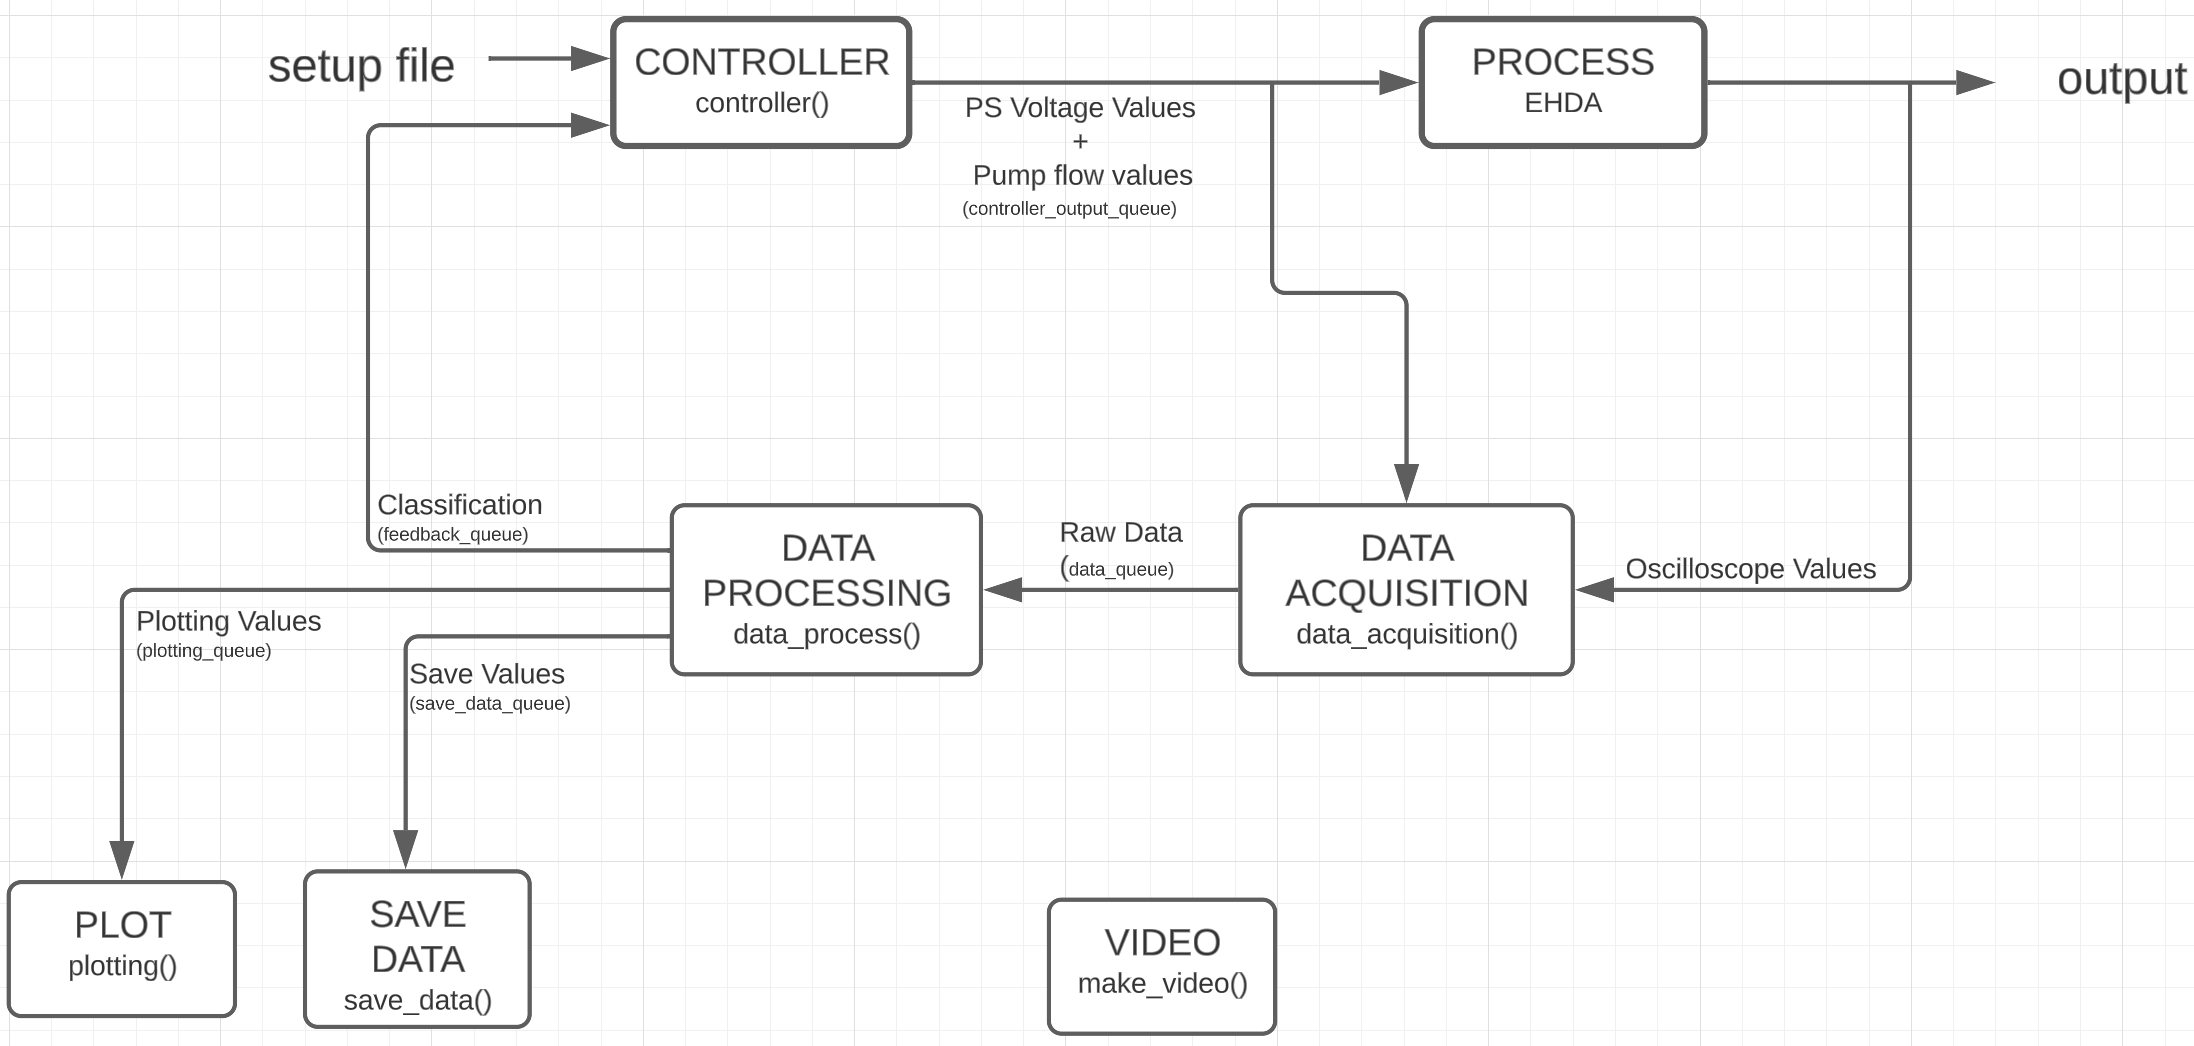
\includegraphics[width=18cm]{images/image_folder_report_4/control_loop.png}
        \caption{Control model implemented in software}
    \end{figure}


\subsection*{2.2 Saved Data Structure}

    With the new streamming model of saving a new structure of the collected data were created.
    Instead of having all data measurements values and after all data processing values we now are saving for each sample the measurements and processing values.
    The structure of the 

    \begin{figure}[H]
        \center
        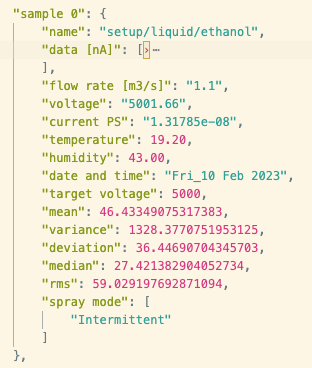
\includegraphics[width=5cm]{images/image_folder_report_4/json_structure.png}
        \caption{Output data json structure}
    \end{figure}

    To work with this data I'm using pandas Dataframe.
    With the command:
    
    pandas.read\textunderscore{}json("PATH", orient='index').

    The json file is good to store the data and to read the file. But as it is getting a lot of data working with pandas Dataframe is being way faster. Also saving the dataframe in a compressed
    type of file called feather is much faster to work with the data.




\subsection*{2.3 Mapping experiments}



    \begin{figure}[H]
        \center
        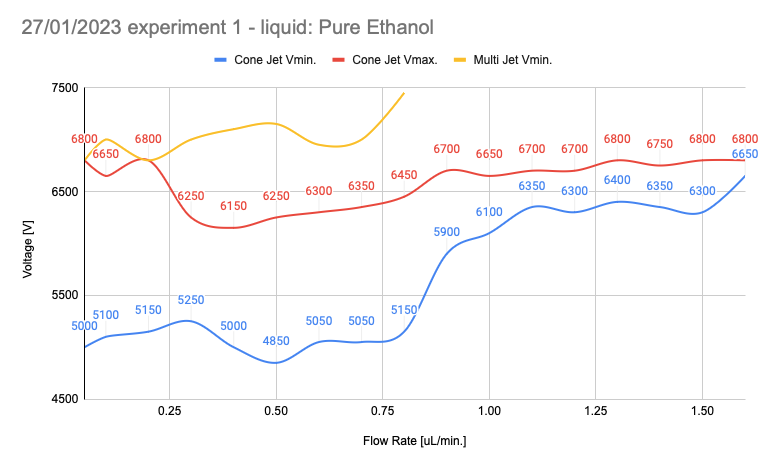
\includegraphics[width=10cm]{images/image_folder_report_4/manualMap1.png}
        \caption{Control model implemented in software}
    \end{figure}

    \begin{figure}[H]
        \center
        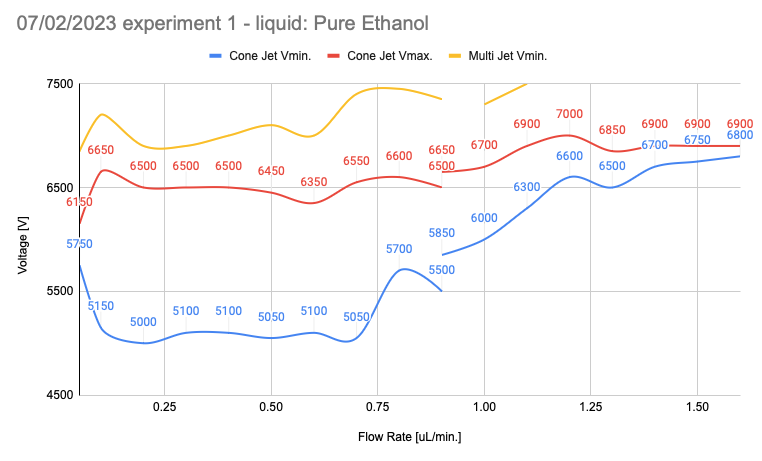
\includegraphics[width=10cm]{images/image_folder_report_4/manualMap2.png}
        \caption{Control model implemented in software}
    \end{figure}

    \begin{figure}[H]
        \center
        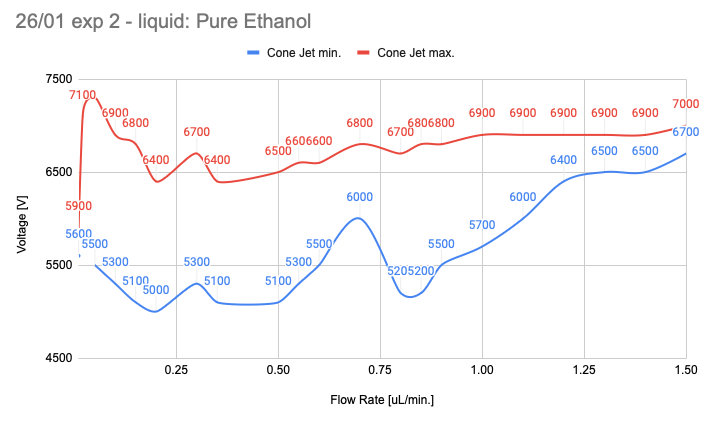
\includegraphics[width=10cm]{images/image_folder_report_4/manualMap3.png}
        \caption{Control model implemented in software}
    \end{figure}


\subsection*{2.4 Manual x Automatic Mapping}


    \begin{figure}[H]
        \center
        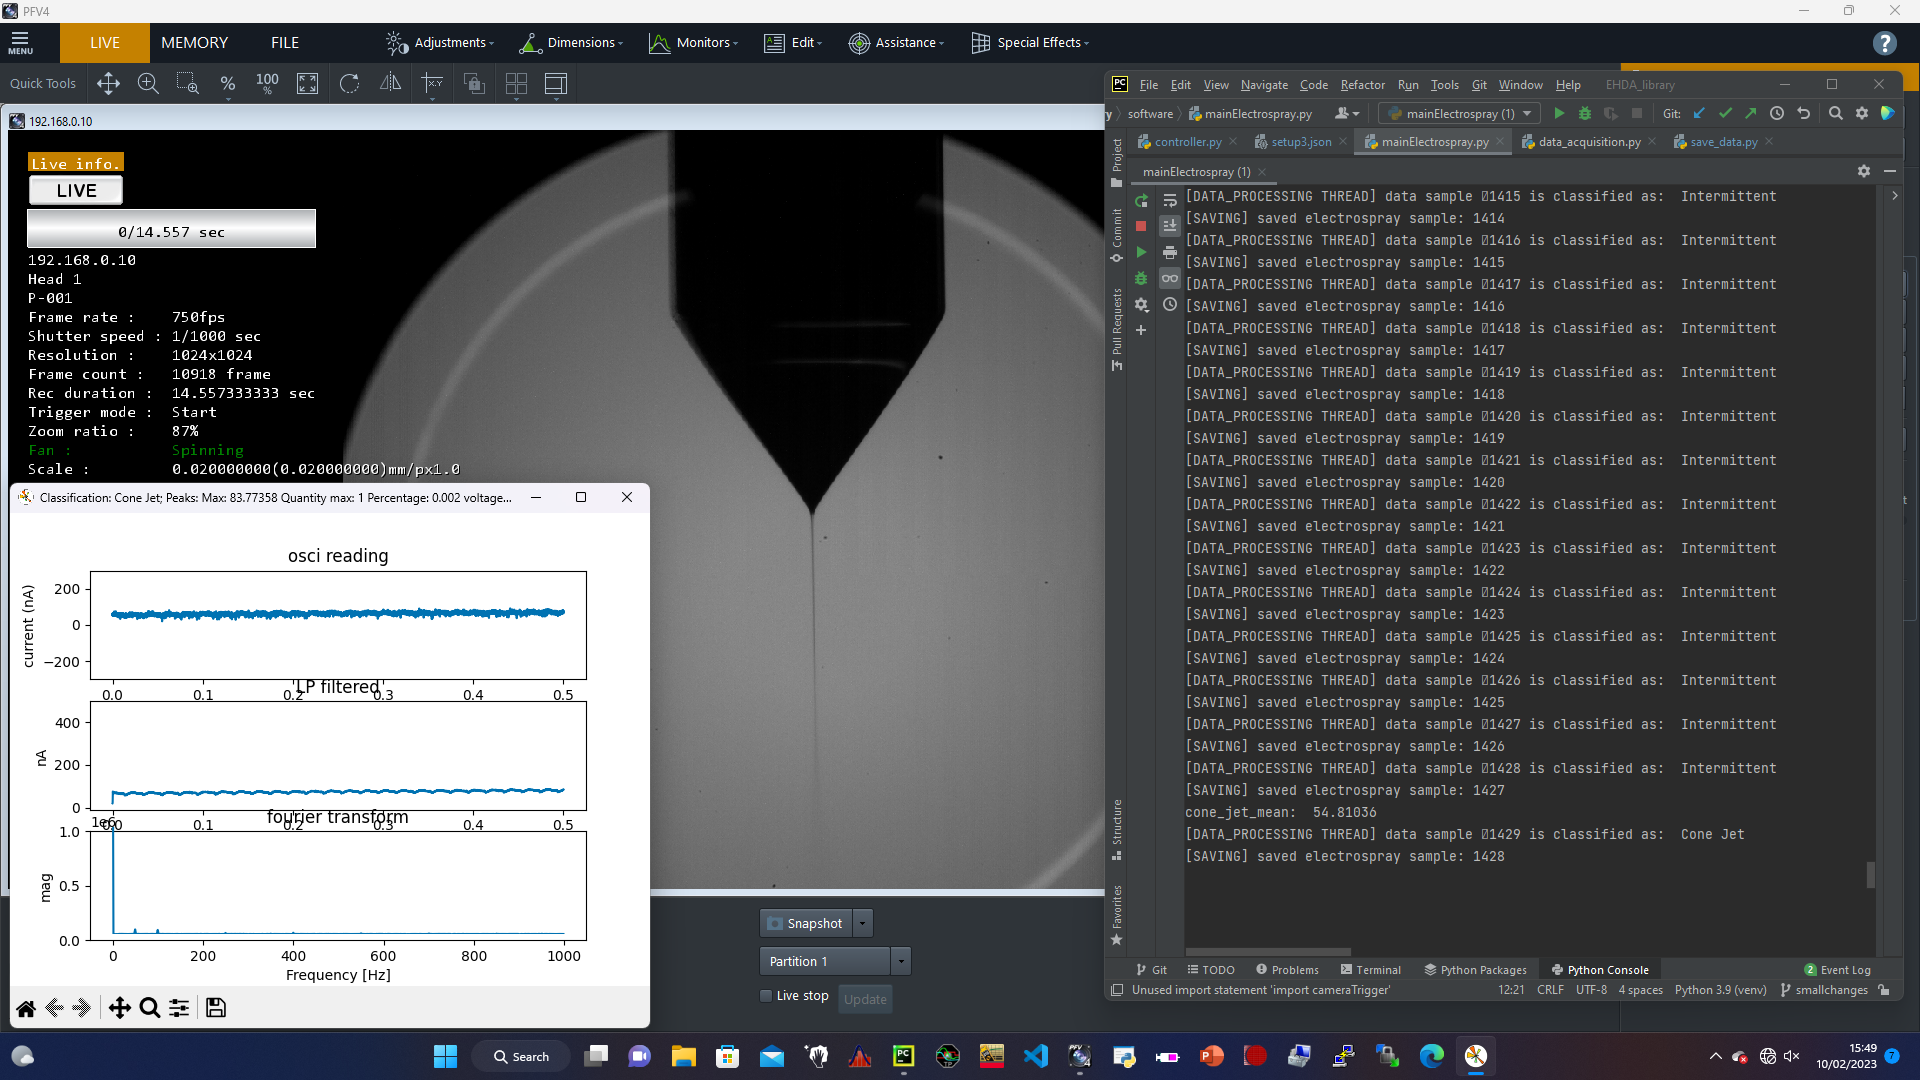
\includegraphics[width=15cm]{images/image_folder_report_4/experiment_print1.png}
        \caption{Control model implemented in software}
    \end{figure}

    \begin{figure}[H]
        \center
        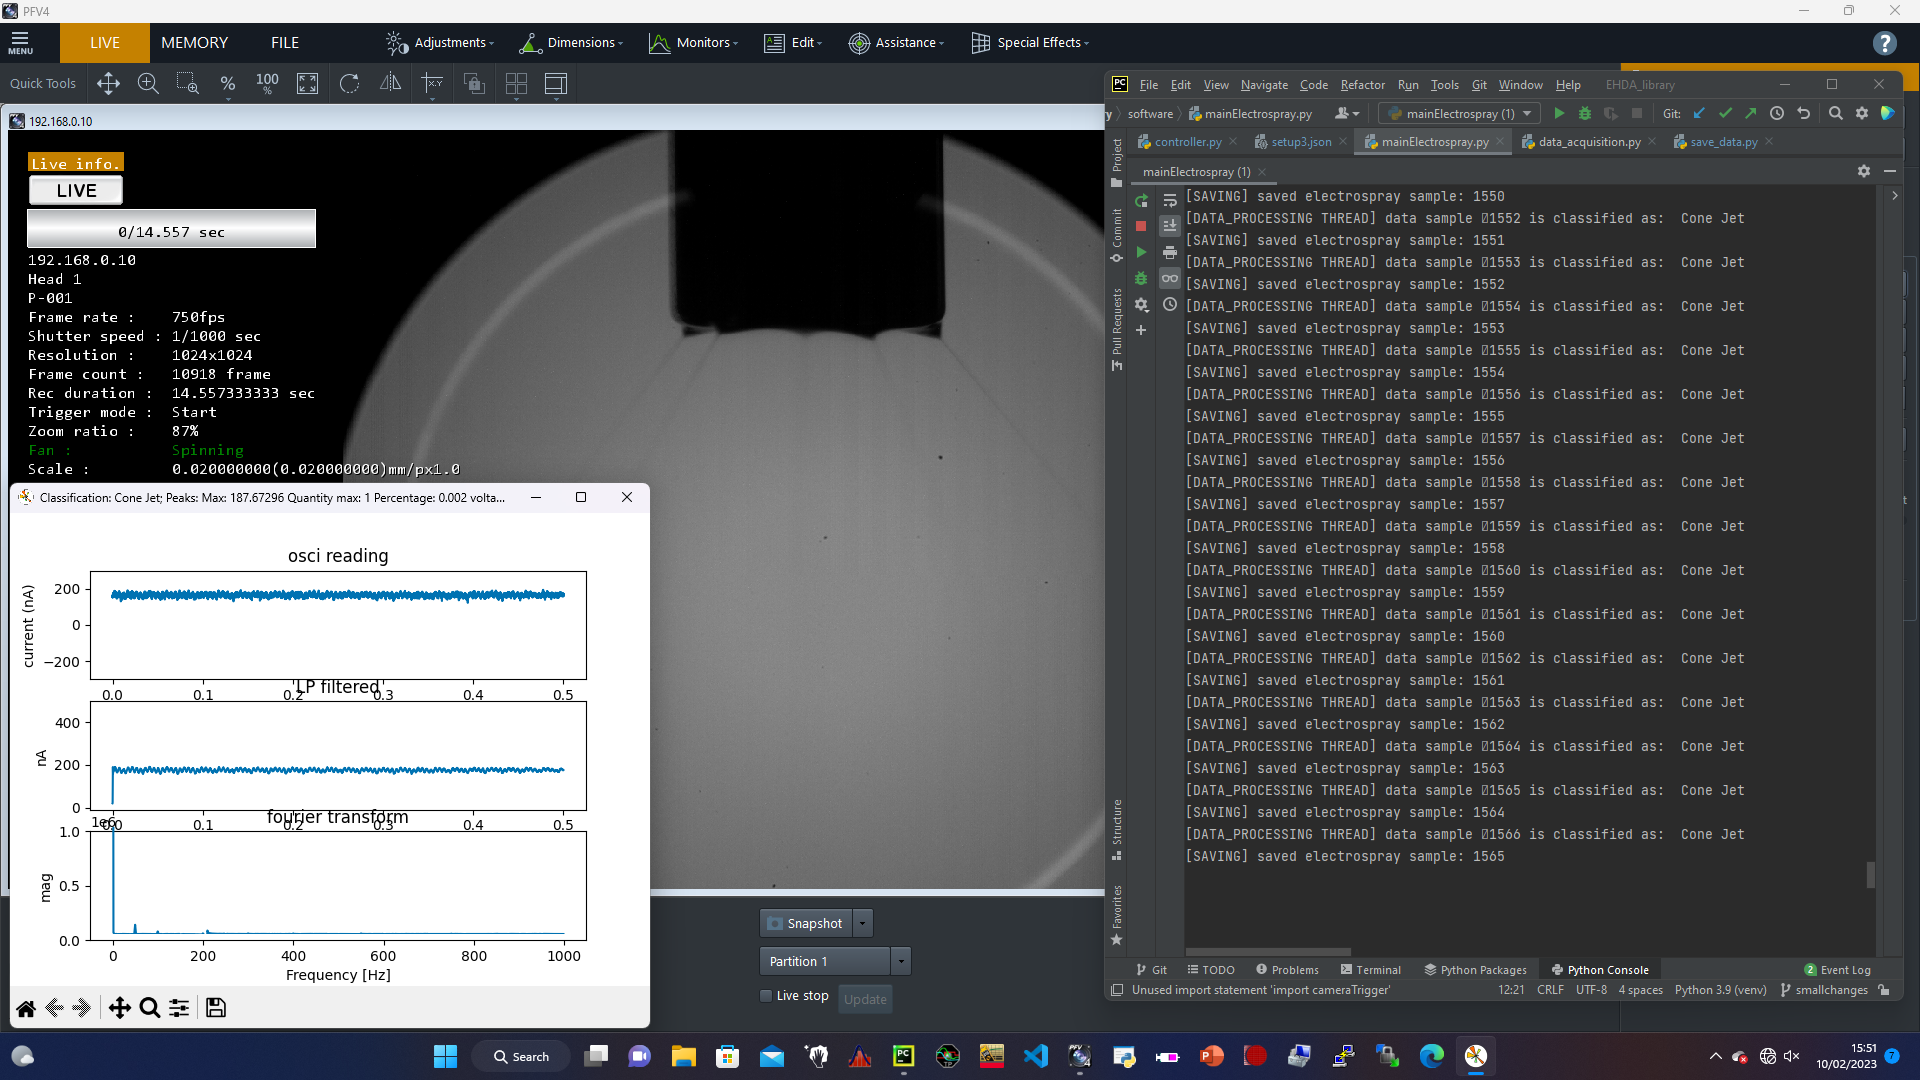
\includegraphics[width=15cm]{images/image_folder_report_4/multi_jet_print.png}
        \caption{Control model implemented in software}
    \end{figure}


    \begin{figure}[H]
        \center
        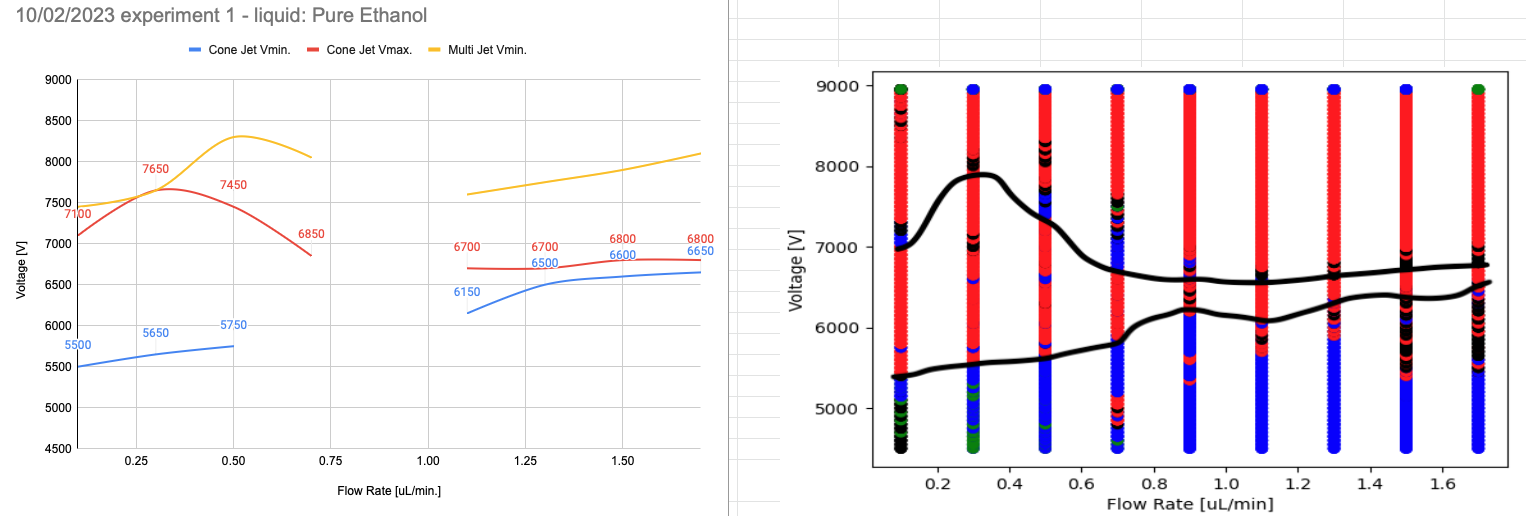
\includegraphics[width=15cm]{images/image_folder_report_4/mapXman-1.png}
        \caption{Control model implemented in software}
    \end{figure}

    \begin{figure}[H]
        \center
        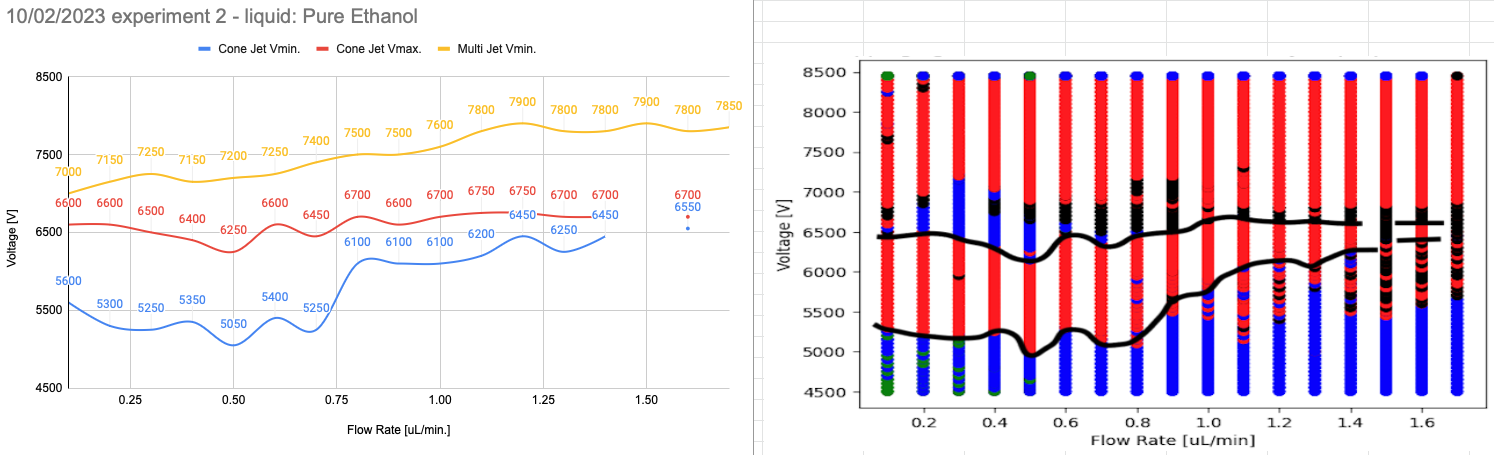
\includegraphics[width=15cm]{images/image_folder_report_4/mapXman-2.png}
        \caption{Control model implemented in software}
    \end{figure}



\subsection*{2.5 Multi Jet classification by mean value}

    There is not many articles about the multi jet dynamics and classification. This makes sometimes hard to define when
    is in multi jet mode, if its defined by the meniscus, quantity of jets or stability.

    We therefore know that the multijet current mean value is above of the cone jet mean value.\cite{Ryan}. This current mean value
    increases for each new jet created. This could also be noticed experimentally in our setup.

    For that, in our automatic classification algorithm, as the current acquired in cone jet and multi jet has the shape (constant) but different DC values. We decided
    to save the cone jet mean value and multi jet mean values and analyse what is this step.

    Making a statistical analysis in all data collected using the same liquid (ethanol) and setup we found that the Multi jet can be classified when the current is 1.14 the value of the Cone Jet mean.
    I implemented this logic in the automatic classification and got the following results.

    \begin{figure}[H]
        \center
        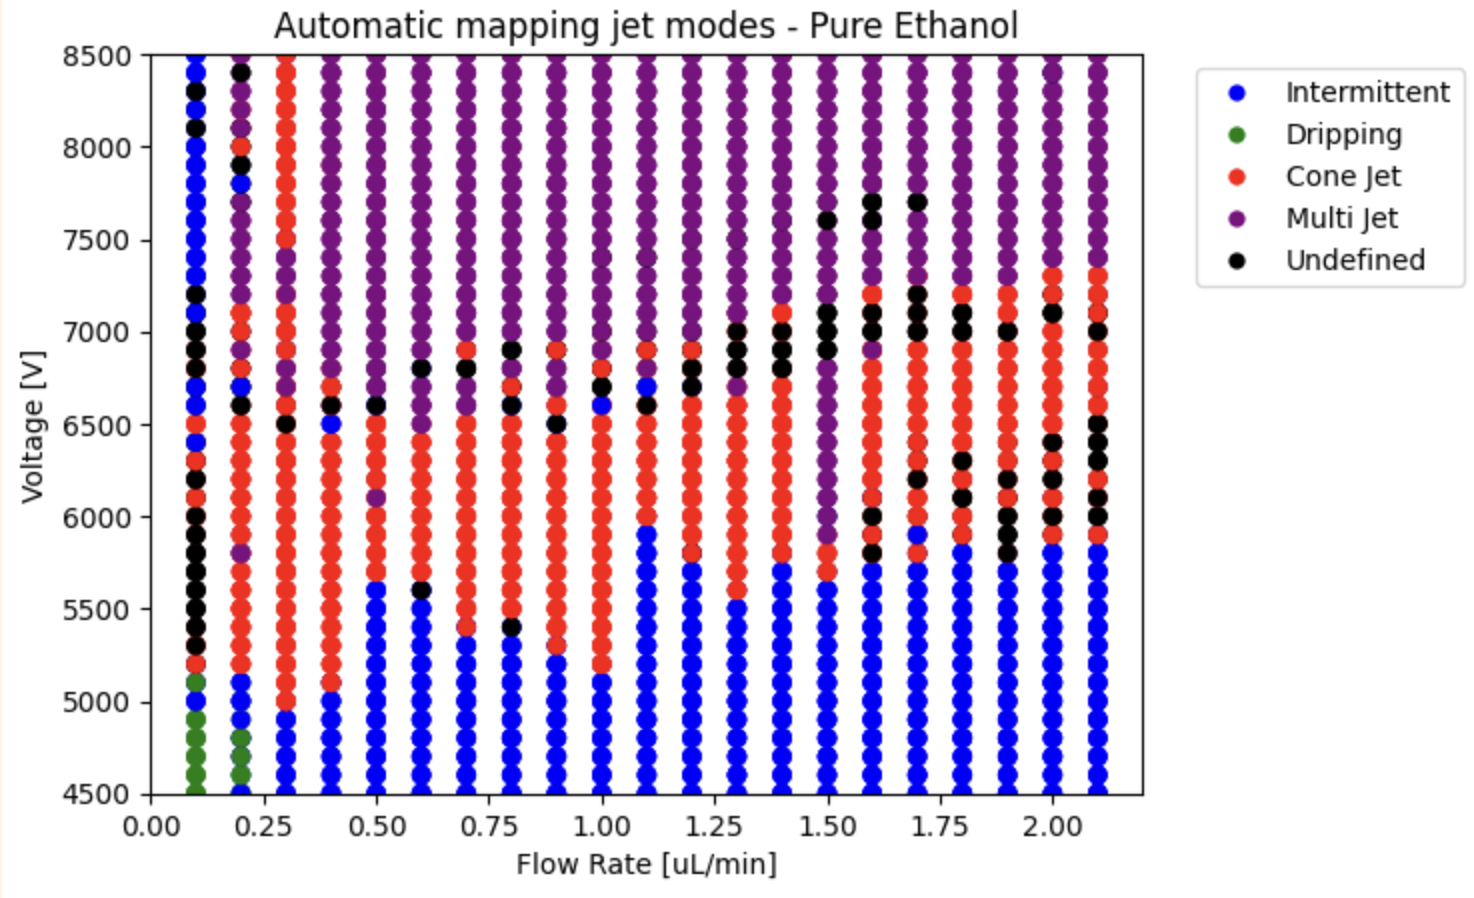
\includegraphics[width=15cm]{images/image_folder_report_4/map7-automatic.png}
        \caption{Control model implemented in software}
    \end{figure}


    Comparing this results with the manual results of the same experiment we can see that the algorithm could classify the Multi Jet with a good accuracy.

    \begin{figure}[H]
        \center
        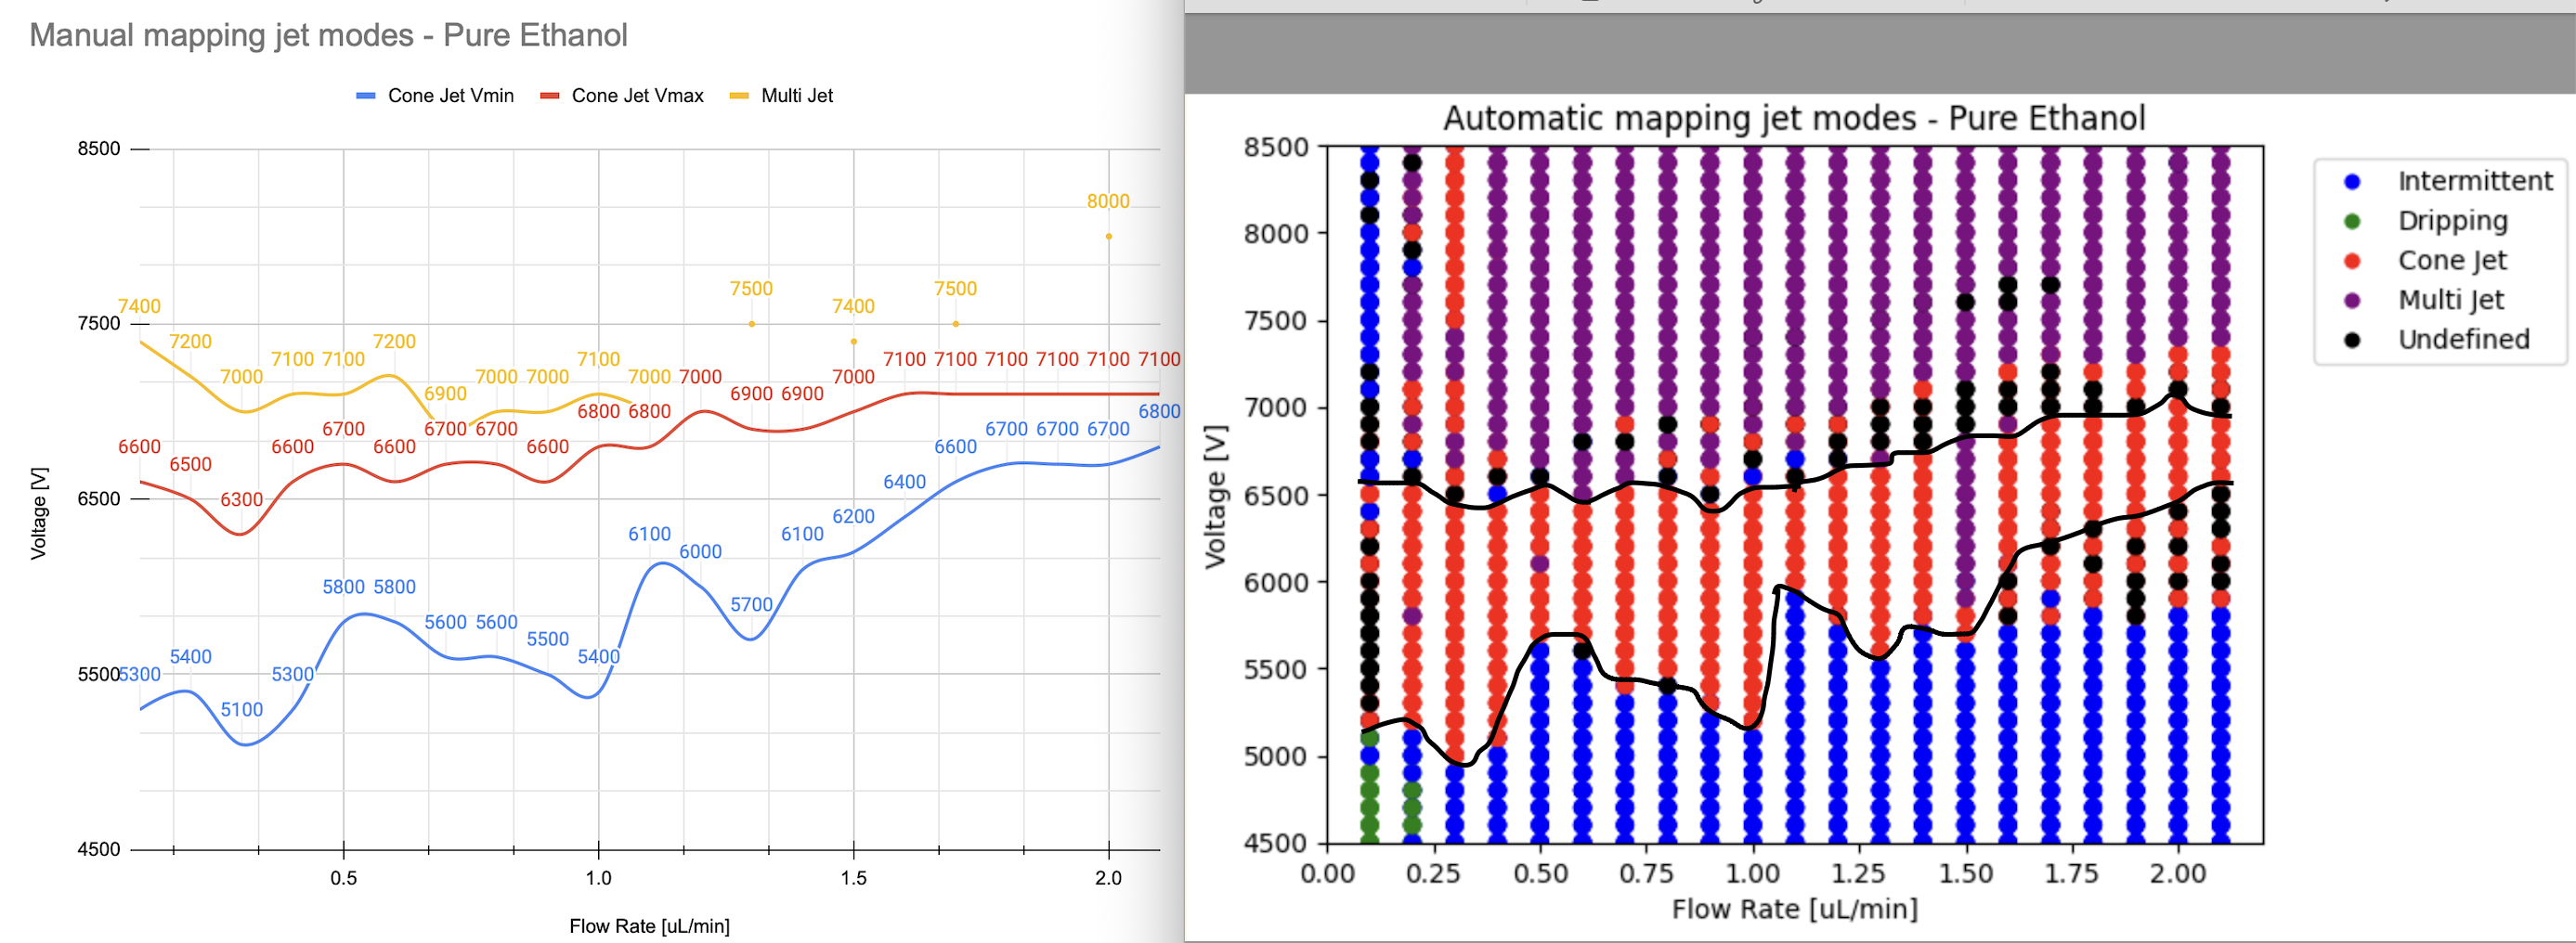
\includegraphics[width=18cm]{images/image_folder_report_4/map7-comparison.png}
        \caption{Control model implemented in software}
    \end{figure}



\subsection*{2.1 Raspberry pi}

As we can see in Figure 4 the plotting thread can simply be deactivated by a command in the configuration file.
With that we are capable of running the routine in a raspberry pi with python3 installed.
The raspberry pi offers the portable solution for the routine to be running and can be implemented in size constrained industries applications.
The raspberry pi is also integrated with a GSM data module to connect in internet through cellphone network.
